\section{Modeling}

\subsection*{Equations}

\begin{frame}
\frametitle{Equations of motion}

\begin{block}{Euler--Lagrangian equations}
\begin{equation*}
 T =\frac{1}{2}\left[m_w(\dot{x_w}^2 + \dot{y_w}^2) + m_p (\dot{x_p}^2 + \dot{y_p}^2)
  + m_l(\dot{x_l}^2 + \dot{y_l}^2) +  J_w(\dot{\phi} + \dot{\theta})^2
  + J_b\dot{\theta}^2\;\right]
\end{equation*}
\vspace{2mm}
\begin{equation*}
V\:=\: g\:\left[\: m_l\:y_l\:+\: m_w\:y_w\:+\: m_p\:y_p\:\right] + \frac{1}{2}K\:(l - l_0)^2
\end{equation*}
\vspace{2mm}
\begin{equation*}
L = T - V
\end{equation*}
\vspace{2mm}
\begin{equation*}
q = \left[\:x\;\;\;y\;\;\;l\;\;\;\theta\;\;\;\phi\:\right] 
\end{equation*}
\vspace{2mm}
\begin{equation*}
\frac{d}{dt}\left(\frac{\partial\:L}{\partial\:\dot{q_A}}\right) - \frac{\partial\:L}{\partial\:q_A} = Q_A
\end{equation*}
\vspace{2mm}
\begin{equation*}
 Q_A = \sum_{r=1}^m\lambda_r\;\frac{\partial \psi_r}{\partial q_A}
\end{equation*}

\end{block}
\end{frame}

\begin{frame}
\frametitle{Stance Phase}
\begin{block}{Stance Phase}
\begin{itemize}
 \item
  Foot touches the ground when,
  \begin{equation*}
  y(t) = (\;l_{impact} - l_0\;)\:\cos \theta_{impact} + d \sin \theta_{impact}
  \end{equation*}\\[0.1in]
  \item
  Constraint equations,
  \begin{eqnarray*}
    y(t) = (\;l(t) - l_0\;)\:\cos \theta + d \sin \theta\\
    x(t) = x_{f-impact} - (\;l(t) - l_0\;)\:\sin \theta - d \cos \theta
  \end{eqnarray*}
  where
  \begin{equation*}
  x_{f-impact} =  x_{impact} + (\;l_{impact} - l_0\;)\:\sin \theta_{impact} + d \cos \theta_{impact}
  \end{equation*}
  \item
  Phase ends when
  \begin{equation*}
  l(t) = l_0 
  \end{equation*}

  \end{itemize}

\end{block}

\end{frame}


\begin{frame}
\frametitle{Flight Phase}
\begin{block}{Spring Controller}
\begin{itemize}
  \item
  \begin{equation*}
  \ddot{l}(t) = \left\{\begin{array}{ll}
			0 & l(t) \leq (l_0 - \epsilon)\;\;OR\;\;l(t) \geq (l_{max} + \epsilon)\\
			&\\
			l_{accel} & l_0 \leq l(t) \leq \frac{(l_{max} + l_0)}{2}\\
			&\\
			-l_{accel} & \frac{(l_{max} + l_0)}{2} \leq l(t) \leq l_{max}
                      \end{array} \right.
  \label{eqn:4_spring_retract}
  \end{equation*}\\[0.1in]
    \item
    Convert $\ddot{l}(t)$ control law to implementable $\dot{l}(t)$ form\\[0.1in]
   \item 
    Sense $\omega(t)$ with encoders,
    \begin{equation*}
    e(t) = \omega(t) - \omega_d(t)
    \end{equation*}\\[0.1in]
    \begin{equation*}
    U_{l}(t) = K_w\;\omega_d(t) + K_p\;e(t) + K_d\;\frac{d\;e(t)}{dt} + K_i\;\int e(t)\;dt
    \label{eqn:4_l_controller}
    \end{equation*}

\end{itemize}
\end{block}
\end{frame}

\begin{frame}
\frametitle{Spring Phase}
\begin{block}{Constrainted flight phase}
\begin{itemize}
  \item
  Constraint is,
  \begin{equation*}
  l(t) = l_{max}
  \end{equation*}
  \item
  Solver stops when,
  \begin{equation*}
  y(t) = (\;l(t) - l_0\;)\:\cos \theta + d \sin \theta
  \end{equation*}

\end{itemize}
\end{block}
\vspace{0.1in}
\begin{figure}
\centering
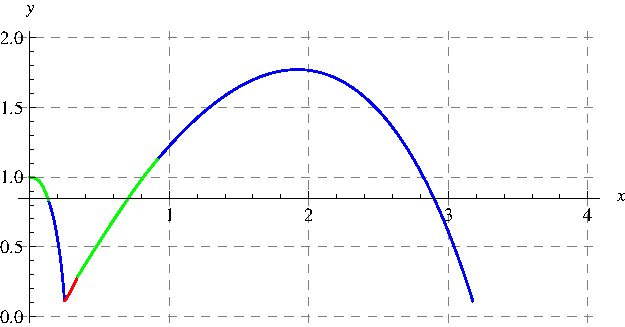
\includegraphics[width=0.7\textwidth]{fig/plotG.pdf}
\caption{Equations of motion propagation}
\end{figure}
\end{frame}

\subsection*{Initial Conditions}
\begin{frame}
\frametitle{Initial Conditions}
\begin{itemize}
  \item 
  Topmost point of the trajectory,\\ i.e. $x = 0$, $\dot{x} = 1$, $\dot{y} = 0$, $y = 1$, $\phi$ is constrained\\[0.1in]
  \item
  Calculate the amount of energy lost in the impact to give $l_{max} = 0.37 m$\\[0.1in]
  \item
  Vary $\theta_0$ and $\dot{\theta}_0$ to minimize norm\\[0.1in]
  \item
  Define norm as,
  \begin{equation*}
  norm = \sum_{i = 1, i\;\neq\;1, 5, 10}^{10} || q_{A_i} - q_{B_i} ||
  \end{equation*}\\[0.1in]
  Remove $x(t)$, $\phi(t)$ and $\dot{\phi}(t)$ from the norm\\[0.1in]
  \item
  Problems with optimizing algorithm, hence manual search\\[0.1in]
  \item
  $\theta_0 = 0$ and $\dot{\theta}_0 = -0.5$ rad/s
\end{itemize}
\end{frame}

% \begin{frame}
% \frametitle{Poincare Map}
% \begin{block}{Linear Poincare Map}
% \begin{itemize}
%   \item 
%   
% \end{itemize}
% 
% \end{block}
% 
% \end{frame}

